\renewcommand{\theequation}{\theenumi}
\begin{enumerate}[label=\thesubsection.\arabic*.,ref=\thesubsection.\theenumi]
\numberwithin{equation}{enumi}
\item 
Find the equation of all lines having slope 2 and being tangent to the curve 
%\cite{twelve_one}
\begin{align}
\label{eq:hyperbola}
y + \frac{2}{x-3} = 0
\end{align}
\solution 
\eqref{eq:hyperbola} can be expressed as
\begin{align}
\label{eq:conic_nofrac}
xy -3y + 2 = 0
\end{align}
which is of the same form as \eqref{eq:conic_quad_form} with 
\begin{align}
\label{eq:hyper_quad_form_param}
\vec{V} = \frac{1}{2}\myvec{0 & 1\\ 1 & 0}, \vec{u} = -\frac{3}{2}\myvec{0 \\1}, f = 2
\end{align}
Using the approach in Example \ref{ex:ellipse_tangent},
\begin{align}
\vec{D} = \myvec{\frac{1}{2} & 0 \\ 0 & -\frac{1}{2}}, \vec{P} = \frac{1}{\sqrt{2}}\myvec{1 & -1\\1 & 1}
\end{align}
\begin{align}
\because \vec{u}^T\vec{V}^{-1}\vec{u}-f = -2 < 0,
\end{align} 
the major and minor axis are swapped and from Table \ref{table:conics}
the hyperbola parameters are given by 
\begin{align}
\vec{c}= 3\myvec{1\\0},
\sqrt{\frac{\vec{u}^T\vec{V}^{-1}\vec{u}-f}{\lambda_2}} = 2,
\\
\sqrt{\frac{f-\vec{u}^T\vec{V}^{-1}\vec{u}}{\lambda_1}} = 2
\end{align}
with the standard hyperbola equation becoming
\begin{align}
\frac{y_2^2}{4}-\frac{y_1^2}{4} = 1,
\label{eq:std_hyper}
\end{align}
%
Fig. \ref{fig:hyper_tangent}	shows  the actual hyperbola in \eqref{eq:hyperbola}  obtained from  
\eqref{eq:std_hyper}  using \eqref{eq:conic_affine}.  
The direction and normal vectors of the tangent with slope 2 are given by \eqref{eq:dir_vec_slope} and \eqref{eq:line_dir_norm} as
\begin{align}
\vec{m} = \myvec{1\\2}, \vec{n} = \myvec{2\\-1}
\end{align}
%
From \eqref{eq:conic_tangent_qk} and \eqref{eq:circle_tangent_prob_uf}, using \eqref{eq:hyper_quad_form_param},
\begin{align}
\kappa = \frac{1}{2}, \vec{q}_1 = \myvec{2\\2}, \vec{q}_2 = \myvec{4\\-2}.
\end{align}
%
The desired tangents are
\begin{align}
\myvec{2 & -1}\cbrak{\vec{x}-\myvec{2\\2}} &= 0 \implies \myvec{2 & -1} \vec{x} = 2
\\
\myvec{2 & -1}\cbrak{\vec{x}-\myvec{4\\-2}} &= 0 \implies \myvec{2 & -1} \vec{x} = 10
\end{align}
All the above results are verified in Fig. \ref{fig:hyper_tangent}.  As we can see, the hyperbola in \eqref{eq:hyperbola} is obtained by rotating the standard hyperbola by $\vec{P}$	and then translating it by $\vec{c}$.

\begin{figure}[!ht]
\centering
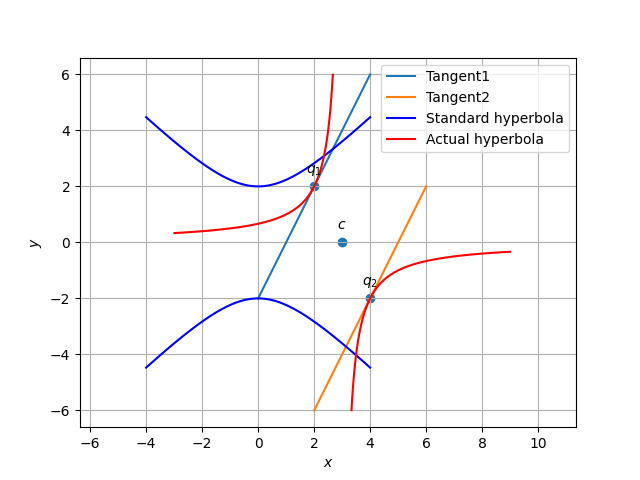
\includegraphics[width=\columnwidth]{./figs/hyper/hyper_tangent.eps}
\caption{Standard and actual hyperbola.}
\label{fig:hyper_tangent}	
\end{figure}
\item Find the asymptotes of the hyperbola given below and also the equations to their conjugate hyperbolas.
\begin{align}
\label{eq:hyper_asymp}
8x^2+10xy-3y^2-2x+4y-2=0
\end{align}
\begin{enumerate}
\item  \eqref{eq:hyper_asymp} can be expressed as \eqref{eq:conic_quad_form} with 
\begin{align}
    \vec{V}=\vec{V}^T&=\myvec{8 & 5 \\ 5 &-3}\label{eq:solutions/40/7/eqv}\\
    \vec{u}&=\myvec{-1 \\2 }\label{eq:solutions/40/7/equ}\\
    f&=-2\label{eq:solutions/40/7/eqfv}
\end{align}   
Expanding the Determinant of $\vec{V}$,
\begin{align}
    \Delta_{V} &= \mydet
%\begin{array}{|cc|}
{
8 &5
\\
5 & -3
}
= -49 < 0
%\end{array}<0
\label{eq:solutions/40/7/eq:hyp}
\end{align}
Hence from \eqref{eq:conic_hyper_cond} and \eqref{eq:solutions/40/7/eq:hyp}, \eqref{eq:hyper_asymp}
%\eqref{eq:solutions/40/7/eq:hyp} 
represents a hyperbola.
The characteristic equation of $\vec{V}$ is obtained by evaluating the determinant 
\begin{align}
%       \begin{array}{|c|}
\mydet{V-\lambda\vec{I}} = 0
\\
%\end{array}&=0\\
%   \begin{array}{|cc|}
\mydet{
8-\lambda & 5 \\ 5 & -3-\lambda
} = 0
\\
%\end{array}&=0\\
    \brak{8-\lambda}\brak{-3-\lambda}-25=0\\
\implies \lambda^2 -5\lambda -49 = 0
\label{eq:asymptotes_char}
\\
    \lambda_{1}= \frac{5+\sqrt{221}}{2}\label{eq:solutions/40/7/eq:matrix_l1}\\
    \lambda_{2}= \frac{5-\sqrt{221}}{2}\label{eq:solutions/40/7/eq:matrix_l2}
\end{align}
The eigenvector $\vec{p}$ is defined as 
\begin{align}
    \vec{V}\vec{p}&=\lambda\vec{p}\\
    \implies (\vec{V}-\lambda\vec{I})\vec{p}&=0\label{eq:solutions/40/7/eq:7/eqev}
\end{align}
For $\lambda_1=\frac{5+\sqrt{221}}{2}$ ,
\begin{align}
    (\vec{V}-\lambda_1\vec{I})=\myvec{\frac{11-\sqrt{221}}{2} & 5 \\5 & \frac{-11-\sqrt{221}}{2}}
\end{align}
By row reduction, 
\begin{align}
    &\myvec{\frac{11-\sqrt{221}}{2} & 5 \\5 & \frac{-11-\sqrt{221}}{2}}\\
    %&\xleftrightarrow{\frac{R_1}{\frac{\sqrt{533}+2}{2}}}\\
%    &\xleftrightarrow{R_1\leftarrow R_2}
%    \myvec{\frac{-11-\sqrt{221}}{2} & 5 \\ \frac{11-\sqrt{221}}{2} & 5}\\
 &\xleftrightarrow{R_2\leftarrow R_2+\frac{11+\sqrt{221}}{10}R_{1}}
    \myvec{5 & \frac{-11-\sqrt{221}}{2} \\ 0& 0}%\\
%     &\xleftrightarrow{R_1\leftarrow R_1/5}
%    \myvec{1 & \frac{-11-\sqrt{221}}{10} \\ 0& 0}
    \label{eq:solutions/40/7/eq:7/eqs1}
\end{align}
Substituting \eqref{eq:solutions/40/7/eq:7/eqs1} in \eqref{eq:solutions/40/7/eq:7/eqev} we get
\begin{align}
        & \myvec{5 & \frac{-11-\sqrt{221}}{2} }\vec{p}_1=\vec{0}
\\
\implies \vec{p}_1 &= k \myvec{ \frac{11+\sqrt{221}}{2} \\ 5}
\label{eq:solutions/40/7/eq:7/eqei1}
\end{align}
For $\lambda_2=\frac{5-\sqrt{221}}{2}$ ,
\begin{align}
    (\vec{V}-\lambda_2\vec{I})=\myvec{\frac{11+\sqrt{221}}{2} & 5 \\5 & \frac{-11+\sqrt{221}}{2}}
\end{align}
By row reduction , 
\begin{align}
     \myvec{\frac{11+\sqrt{221}}{2} & 5 \\5 & \frac{-11+\sqrt{221}}{2}}
\\
    \xleftrightarrow{R_2\leftarrow R_2+ \frac{11-\sqrt{221}}{10}R_1}
     \myvec{\frac{11+\sqrt{221}}{2} &5\\ 0& 0}
    \label{eq:solutions/40/7/eq:es71/eqs2}
\end{align} 
Substiuting \eqref{eq:solutions/40/7/eq:es71/eqs2} in \eqref{eq:solutions/40/7/eq:7/eqev} we get 
\begin{align}
     \myvec{\frac{11+\sqrt{221}}{2} &5}\vec{p}_2=\vec{0}
\\
\implies \vec{p}_2 &= k \myvec{ -5 \\ \frac{11+\sqrt{221}}{2}}
\label{eq:solutions/40/7/eq:es71/eqei2}
\end{align}
Thus, we obtain 
\begin{align}
\vec{P} &= \myvec{\vec{p}_1 & \vec{p}_2}
= k \myvec{ \frac{11+\sqrt{221}}{2} & -5  \\ 5 & \frac{11+\sqrt{221}}{2}}
\end{align}
%
For
\begin{align}
\vec{P}^{\top}\vec{P} &= \vec{I},
k = \sqrt{\frac{221+11\sqrt{221}}{2}}
\end{align}
\begin{multline}
\implies \vec{P} = \sqrt{\frac{2}{221+11\sqrt{221}}}
\\
\times \myvec{ \frac{11+\sqrt{221}}{2} & -5  \\ 5 & \frac{11+\sqrt{221}}{2}}
\label{eq:solutions/40/7/eq:es71/eqP}
\end{multline}
and
\begin{align}
    \vec{V}&=\vec{P}\vec{D}\vec{P}^T\label{eq:solutions/40/7/eq:es71/eqsubs}
\end{align}
where 
\begin{align}
       \vec{D}&=\myvec{\frac{5+\sqrt{221}}{2} & 0\\0 & \frac{5-\sqrt{221}}{2}}\label{eq:solutions/40/7/eq:es71/eqDD}
\end{align}
Centre of the hyperbola is given by 
\begin{align}
    \vec{c}&=-\vec{V}^{-1}\vec{u}\\
    \implies\vec{c}&=-\myvec{\frac{3}{49}&\frac{5}{49}\\\frac{5}{49}&\frac{-8}{49}}\myvec{-1 \\ 2}\\
    \implies\vec{c}&=\myvec{\frac{-3}{49}&\frac{-5}{49}\\\frac{-5}{49}&\frac{8}{49}}\myvec{-1 \\ 2}\\
    \implies\vec{c}&=\myvec{\frac{-1}{7}\\\frac{3}{7}}
\end{align}
Since,
\begin{align}
    \vec{u}^T\vec{V}^{-1}\vec{u}-f = 1 > 0\label{eq:solutions/40/7/eq:es71/cond}
\end{align} 
there isn't a need to swap axes
In hyperbola,
\begin{align}
axes=
\begin{cases}
\sqrt{\frac{\vec{u}^T\vec{V}^{-1}\vec{u}-f}{\lambda_1}}\\ \sqrt{\frac{f-\vec{u}^T\vec{V}^{-1}\vec{u}}{\lambda_2}}
\end{cases}
\end{align}
From above equations we can say that,
\begin{align}
\sqrt{\frac{\vec{u}^T\vec{V}^{-1}\vec{u}-f}{\lambda_1}}=\sqrt{ \frac{2}{5+\sqrt{221}}}\\
\sqrt{\frac{f-\vec{u}^T\vec{V}^{-1}\vec{u}}{\lambda_2}}=\sqrt{ \frac{2}{5-\sqrt{221}}}
\end{align}
The equation of the hyperbola at the origin is then given by \eqref{eq:conic_simp_temp_nonparab} as
 %Now we have,
\begin{align}
    \vec{y}^T\vec{D}\vec{y}=\vec{u}^T\vec{V}^{-1}\vec{u}-f\label{eq:solutions/40/7/eq:es71/fi}
\\
   \implies\vec{y}^T\myvec{\frac{5+\sqrt{221}}{2} & 0 \\0 & \frac{5-\sqrt{221}}{2}}\vec{y}= 1
\end{align}
\item ({\em Asymptotes of hyperbola: })
The equation for the asymptotes of \eqref{eq:hyper_asymp} is given by \eqref{eq:asymp_quad_form} with 
\begin{align} 
K &=  \vec{u}^T\vec{V}^{-1}\vec{u}
\\
&=   \myvec{-1 & 2 }  \myvec{8 & 5 \\ 5 &-3}^{-1}\myvec{-1 \\2 }
 =-1
\label{eq:quad_form_asymp_condK}
\end{align}
%
From \eqref{eq:quad_form_pair_normvecs}, \eqref{eq:solutions/40/7/eq:matrix_l1} and \eqref{eq:solutions/40/7/eq:matrix_l2},
%
\begin{multline}
\vec{n}_1 =  \sqrt{\frac{2}{221+11\sqrt{221}}}
\\
\times \myvec{ \frac{11+\sqrt{221}}{2} & 5  \\ -5 & \frac{11+\sqrt{221}}{2}}
\\
\times \myvec{\sqrt{\frac{\sqrt{221}+5}{2}} \\  \sqrt{\frac{\sqrt{221}-5}{2}}}
%\label{eq:solutions/40/7/eq:es71/eqP}
\end{multline}
%
which can be expressed as
%
\begin{multline}
\vec{n}_1 = 
 \frac{1}{\sqrt{\brak{\lambda+3}^2+5^2}}
\\
\times \myvec{ \lambda_1+3 & 5  \\ -5 & \lambda_1+3}
\myvec{\sqrt{\lambda_1} \\  \frac{7}{\sqrt{\lambda_1}}}
%\label{eq:solutions/40/7/eq:es71/eqP}
\end{multline}
%
which is equivalent to
%
\begin{align}
\vec{n}_1 &= 
\myvec{ \lambda_1+3 & 5  \\ -5 & \lambda_1+3}\myvec{\lambda_1 \\  7}
\\
&= \myvec{ \lambda^2_1+3\lambda_1 +35  \\ 2\lambda_1 +21}
\\
&= \myvec{ 8\lambda_1 +84  \\ 2\lambda_1 +21}
%\label{eq:solutions/40/7/eq:es71/eqP}
\end{align}
using \eqref{eq:asymptotes_char}, which is equivalent to
\begin{align}
\vec{n}_1 &= \myvec{4 \\ 1}
\end{align}
%
Similarly, it can be shown that 
\begin{align}
\vec{n_2}&=\myvec{2\\3} \label{eq:solutions/40/7/eq:normal1}
\end{align}
%
%\item {Conjugate Hyperbola: }  The angle between the asymptotes is obtained from \eqref{eq:solutions/40/7/eq:matrix_l1} and \eqref{eq:solutions/40/7/eq:matrix_l2} as
%\begin{align}
%	\cos\theta=\brak{\frac{5}{\sqrt{221}}},
%	\sin\theta=\brak{\frac{14}{\sqrt{221}}}
%\end{align}
%%
%Consequently, the rotation matrix 
%\begin{align}
%\label{eq:asymp_conj_rot_mat}
%\vec{Q} = \frac{1}{\sqrt{221}}\myvec{
%5 & -14
%\\
%14 & 5
%} 
%\end{align}
%and the conjugate hyperbola is obtained from 
%\eqref{eq:hyper_asymp} and  \eqref{eq:conic_quad_form_conjugate}.
%as 
%
Fig.     \ref{eq:solutions/40/7/Fig :1} plots the hyperbola in \eqref{eq:hyper_asymp} along with the asymptotes obtained using \eqref{eq:quad_form_pair}.
 

\begin{figure}[!ht]
    \centering
    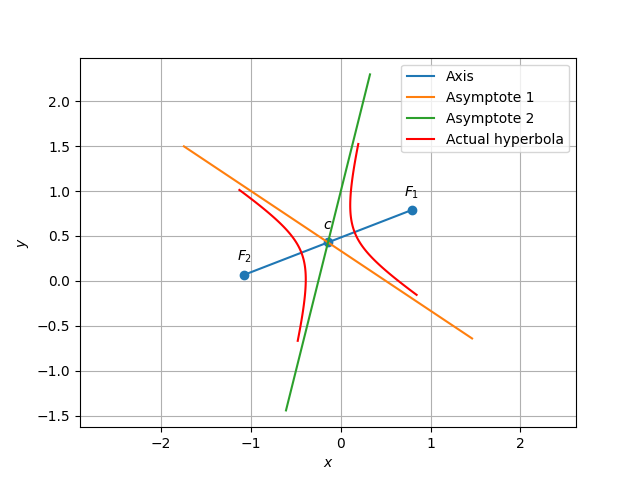
\includegraphics[width=\columnwidth]{./figs/asymp/hyper_asymp.png}
    \caption{Hyperbola with assymptotes and its conjugate}
    \label{eq:solutions/40/7/Fig :1}
\end{figure}
\end{enumerate}

\end{enumerate}
